\documentclass{beamer}
\usetheme{Madrid}
\usepackage{tikz}
\usepackage[english]{babel}  % Подключение для автоматического переноса слов

\title{Osint Bot Presentation}
\author{CEO | Yana Anisimova}


\begin{document}

\frame{\titlepage}

\section{What's the problem? Our people may be working for the enemy without even realizing it}

\begin{frame}
  \frametitle{\small What's the problem? Our people may be working for the enemy without even realizing it}
  \sloppy  % Добавлено для избежания переполнений
  \begin{itemize}
    \item Is the company I am going to work for connected to the aggressor country?
    \item Is it a reliable company?
    \item Is it worth getting involved with?
    \item Will I have problems because I work or worked for this company?
    \item Etc.
  \end{itemize}
\end{frame}

\section{AI-based Telegram bot that checks employer using OSINT methods}

\begin{frame}
  \frametitle{\small AI-based Telegram bot that checks employer using OSINT methods}
  \begin{itemize}
    \item Find job postings of your employer on .ru and .by websites
    \item Analyze employer connections with the aggressor country using OSINT methods
  \end{itemize}
  
  \begin{center}
  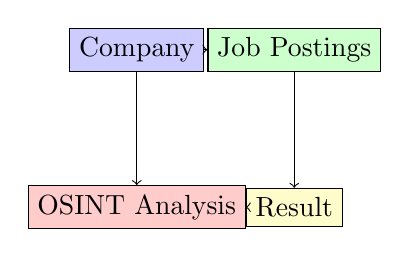
\begin{tikzpicture}[node distance=2cm, auto]
    % Nodes
    \node (company) [rectangle, draw, fill=blue!20] {Company};
    \node (job) [rectangle, draw, right of=company, fill=green!20] {Job Postings};
    \node (osint) [rectangle, draw, below of=company, fill=red!20] {OSINT Analysis};
    \node (result) [rectangle, draw, right of=osint, fill=yellow!20] {Result};

    % Arrows
    \draw[->] (company) -- (job);
    \draw[->] (company) -- (osint);
    \draw[->] (osint) -- (result);
    \draw[->] (job) -- (result);
  \end{tikzpicture}
  \end{center}
\end{frame}



\begin{frame}
    \frametitle{ Market size ukrainian and friends of Ukraine}
  \sloppy  % Добавлено для избежания переполнений

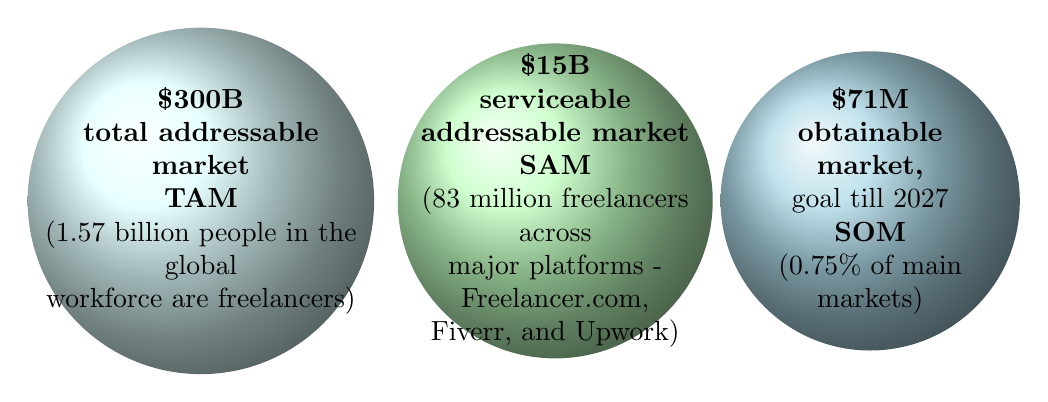
\begin{tikzpicture}

    % Colors for the circles
    \definecolor{lightblue}{RGB}{173,216,230}
    \definecolor{lightgreen}{RGB}{192,255,192}
    \definecolor{lightcyan}{RGB}{224,255,255}
    
    % TAM Circle (уменьшено с 3 до 2.5)
    \shade[ball color=lightcyan] (-5,0) circle (2.2cm);
    \node at (-5,0) {\parbox{4cm}{
        \centering
        \textbf{\$300B}\\
        \textbf{total addressable market}\\
        \textbf{TAM}\\
        (1.57 billion people in the global\\
        workforce are freelancers)
    }};

    % SAM Circle (уменьшено с 2.5 до 2)
    \shade[ball color=lightgreen] (-0.5,0) circle (2cm);
    \node at (-0.5,0) {\parbox{4cm}{
        \centering
        \textbf{\$15B}\\
        \textbf{serviceable addressable market}\\
        \textbf{SAM}\\
        (83 million freelancers across\\
        major platforms - Freelancer.com,\\
        Fiverr, and Upwork)
    }};

    % SOM Circle (уменьшено с 2 до 1.5)
    \shade[ball color=lightblue] (3.5,0) circle (1.9cm);
    \node at (3.5,0) {\parbox{3cm}{
        \centering
        \textbf{\$71M}\\
        \textbf{obtainable market,}\\
        goal till 2027\\
        \textbf{SOM}\\
        (0.75\% of main markets)
    }};
    
\end{tikzpicture}

\end{frame}

\end{document}
